\documentclass[journal,11pt,a4paper]{article}
\usepackage[top = 0.9in,bottom = 0.9in,left = 0.8in,right = 0.8in]{geometry}
\setlength{\columnsep}{1cm}
\usepackage{amssymb}
\usepackage{amsfonts}
\usepackage{amsmath}
\usepackage{amsthm}
\usepackage{setspace}
\usepackage{longtable}
\usepackage{enumitem}
\usepackage{mathtools}
\usepackage{color}                                  
\usepackage{array}
\usepackage{calc} 
\usepackage{bm}
\usepackage{float}
%to fix position (H)
\usepackage{multicol}
%to insert multiple columns
\setlength{\parindent}{0pt}
%no indentation for paragraphs
\begin{document}

\title{ASSIGNMENT-1}
\author{AI21BTECH11021}
\date{March 2022}
\maketitle
\begin{multicols}{2}
\section*{\large Question 3(c)}
\begin{figure}[H]
    \centering
    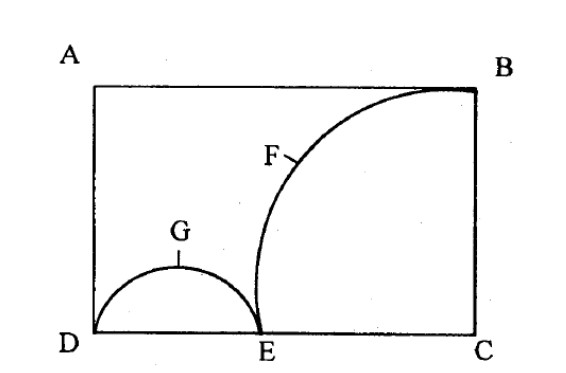
\includegraphics[scale = 0.5]{Figure_1.jpg}
\end{figure}

In the figure given below, ABCD is a rectangle.${AB = 14cm}$ and
${BC= 7 cm}$.From the rectangle, a quarter circle BFEC and a
semicircle DGE are removed.Calculate the area of the remaining
piece of the rectangle?.\\
( Take $ \pi = 22/7 $)\\
\hline
\section*{\Large{Solution\:}}

\begin{table}[H]
    \centering
    \renewcommand{\arraystretch}{1.5}
    \begin{tabular}{|c|p{1.5cm}|p{1.2cm}|p{1.2cm}|}
    \hline
    Shape & Rectangle & semi circle & Quarter circle\\ \hline
    Area &$l*b$ & $\frac{1}{2}\pi r^2$ & $\frac{1}{4}\pi r^2$\\
    \hline
    \end{tabular}
    \caption{Required areas}
\end{table}

\begin{center}
 \begin{align*}
    \text{so area of rectangle ABCD}&= 14cm\times 7cm\\
                 &= 98cm^2.\\
  \end{align*}
\end{center}
\columnbreak
%====================================================================
  \begin{center}
  \begin{align*}
        \text{since BC and EC are the radius of same} circle&\\
    \implies \text{The length of} BC = EC = 7cm.&\\
        \text{since AB and DC are the radius of same circle&}\\
    \implies \text{length& of}AB = DC = 14cm.& \\ 
                     \text{So}\ DE=DC-EC =7cm.& \\ 
\therefore \text{The radius of semicircle GDE} =\frac{DE}{2}=\frac{7}{2}cm&\\
 \end{align*}
    \end{center}
    \vspace{-15pt}
\begin{align*}
\text{Area of BFEC region} &= \frac{1}{4} \times \pi \times 7cm \times 7cm\\ 
               &= \frac{77}{2}cm^2.\text{(radius is BC)}\\
\end{align*}
\vspace{-15pt}
\begin{align*}
\text{Area of GDE region} &=\frac{1}{2} \times \pi \times \frac{7}{2}cm \times \frac{7}{2}cm.\\
                          &= \frac{77}{4}cm^2.\\
\end{align*}
      \vspace{-15pt}
  \begin{flushleft}
Area of required part = area of rectangle - area of semicircle - area of quarter circle.\\
   \end{flushleft}
   \vspace{-15pt}
   \begin{align*}
\implies area required &=98cm^{2} - \frac{77}{2}cm^{2} - \frac{77}{4}cm^{2}\\ 
&= \frac{161}{4}cm^{2} \\
&= 40.25cm^{2}  \\
    \end{align*}
    \vspace{-15pt}
$$ \therefore \text{Area of the region ABFEGD} = 40.25cm^2 $$  
\end{multicols}
\pagebreak
%====================================================================

\rule{\textwidth}{0.4pt}\\
\begin{figure}[h!]
    \centering
    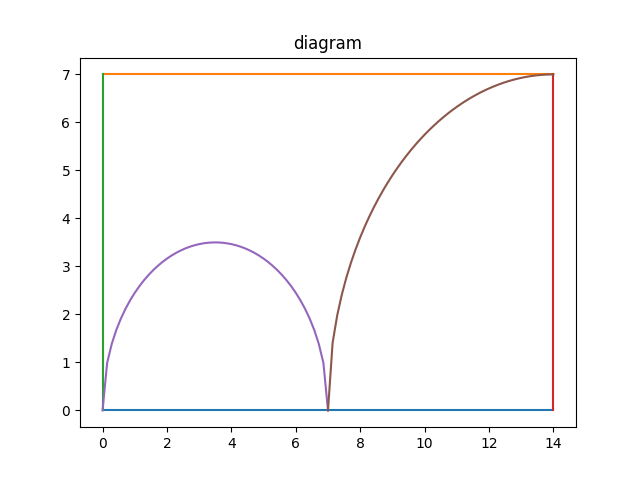
\includegraphics[scale = 0.5]{Figure_2.png}
    \caption{python programmed}
    \label{fig:my_label}
\end{figure}

\rule{\textwidth}{0.4pt}\\
\begin{center}
\textbf{Verification in python}    
\end{center}

\begin{figure}[h!]
    \centering
    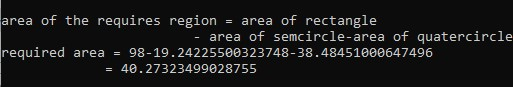
\includegraphics[scale = 0.6]{Figure_3.jpg}
    \caption{python}
    \label{fig:my_label}
\end{figure}

\end{document}
